\documentclass[11pt, a4paper]{article}
\usepackage[utf8]{inputenc}
\usepackage[T1]{fontenc}
\usepackage{geometry}
\geometry{top=1in, bottom=1in, left=1in, right=1in}
\usepackage{graphicx}
\usepackage{float}
\usepackage{xcolor}
\usepackage{amsmath, amssymb}
\usepackage{tcolorbox}
\usepackage{hyperref}
\usepackage{fancyhdr}
\usepackage{helvet}
\renewcommand{\familydefault}{\sfdefault} % Arial/Helvetica-like
\usepackage{setspace}
\setstretch{1.2}

\pagestyle{fancy}
\fancyhf{}
\lhead{DSA5205 Project 2 | Group 28}
\rhead{Buy the Dip Strategy}
\cfoot{\thepage}

\hypersetup{
    colorlinks=true,
    linkcolor=blue,
    filecolor=magenta,      
    urlcolor=cyan,
    pdftitle={Project 2: Buy the Dip Strategy},
}

\begin{document}

\begin{titlepage}
    \centering
    \vspace*{2in}
    {\Large\bfseries DSA5205 Machine Learning in Finance\par}
    \vspace{0.5in}
    {\Large\bfseries Project 2: Design, Validate, and Analyze an Original Asset Trading Strategy\par}
    \vspace{0.3in}
    {\large An Investigation of Mean Reversion, Overfitting Controls, and Dynamic Regime Thresholding\par}
    \vspace{1.5in}
    {\large \textbf{Group 28}\par}
    \vspace{0.2in}
    {\large Institution: National University of Singapore\par}
    \vspace{0.2in}
    {\large Date: October 2026\par}
\end{titlepage}

\newpage
\tableofcontents
\newpage

\section{Introduction \& Economic Story}
. . . . . . . . . . . . . . . . . . . . . . . . . . . . . . . . . . . . . . . . . . . . . . . . . . . . . . . . . . . . . . . . . 4


\subsection{Theoretical Context in Quantitative Finance . . . . . . . . . . . . . . . . . . . . . . . . . . . . . . . . . . . . . . . . . . . . . . . 4}

\subsection{The ``Buy the Dip'' Hypothesis . . . . . . . . . . . . . . . . . . . . . . . . . . . . . . . . . . . . . . . . . . . . . . . . . . . . . . . . . . . . 4}

\subsection{The Role of Machine Learning: Embracing the Virtue of Complexity . . . . . . . . . . . . . . . . . . . . . . 4}

\section{Markets, Assets, and Timing Mechanics}
. . . . . . . . . . . . . . . . . . . . . . . . . . . . . . . . . . . . . . . . . . . . . . . . . . 6


\subsection{Asset Selection: NVIDIA Corporation (NVDA) . . . . . . . . . . . . . . . . . . . . . . . . . . . . . . . . . . . . . . . . . . . 6}

\subsection{Trading Frequency \& Calendar . . . . . . . . . . . . . . . . . . . . . . . . . . . . . . . . . . . . . . . . . . . . . . . . . . . . . . . . . . . . 6}

\subsection{Execution Mechanics \& Elimination of Look-Ahead Bias . . . . . . . . . . . . . . . . . . . . . . . . . . . . . . . . . 7}

\subsection{Investable Benchmarks . . . . . . . . . . . . . . . . . . . . . . . . . . . . . . . . . . . . . . . . . . . . . . . . . . . . . . . . . . . . . . . . . . . . 7}


\begin{figure}[H]
    \centering
    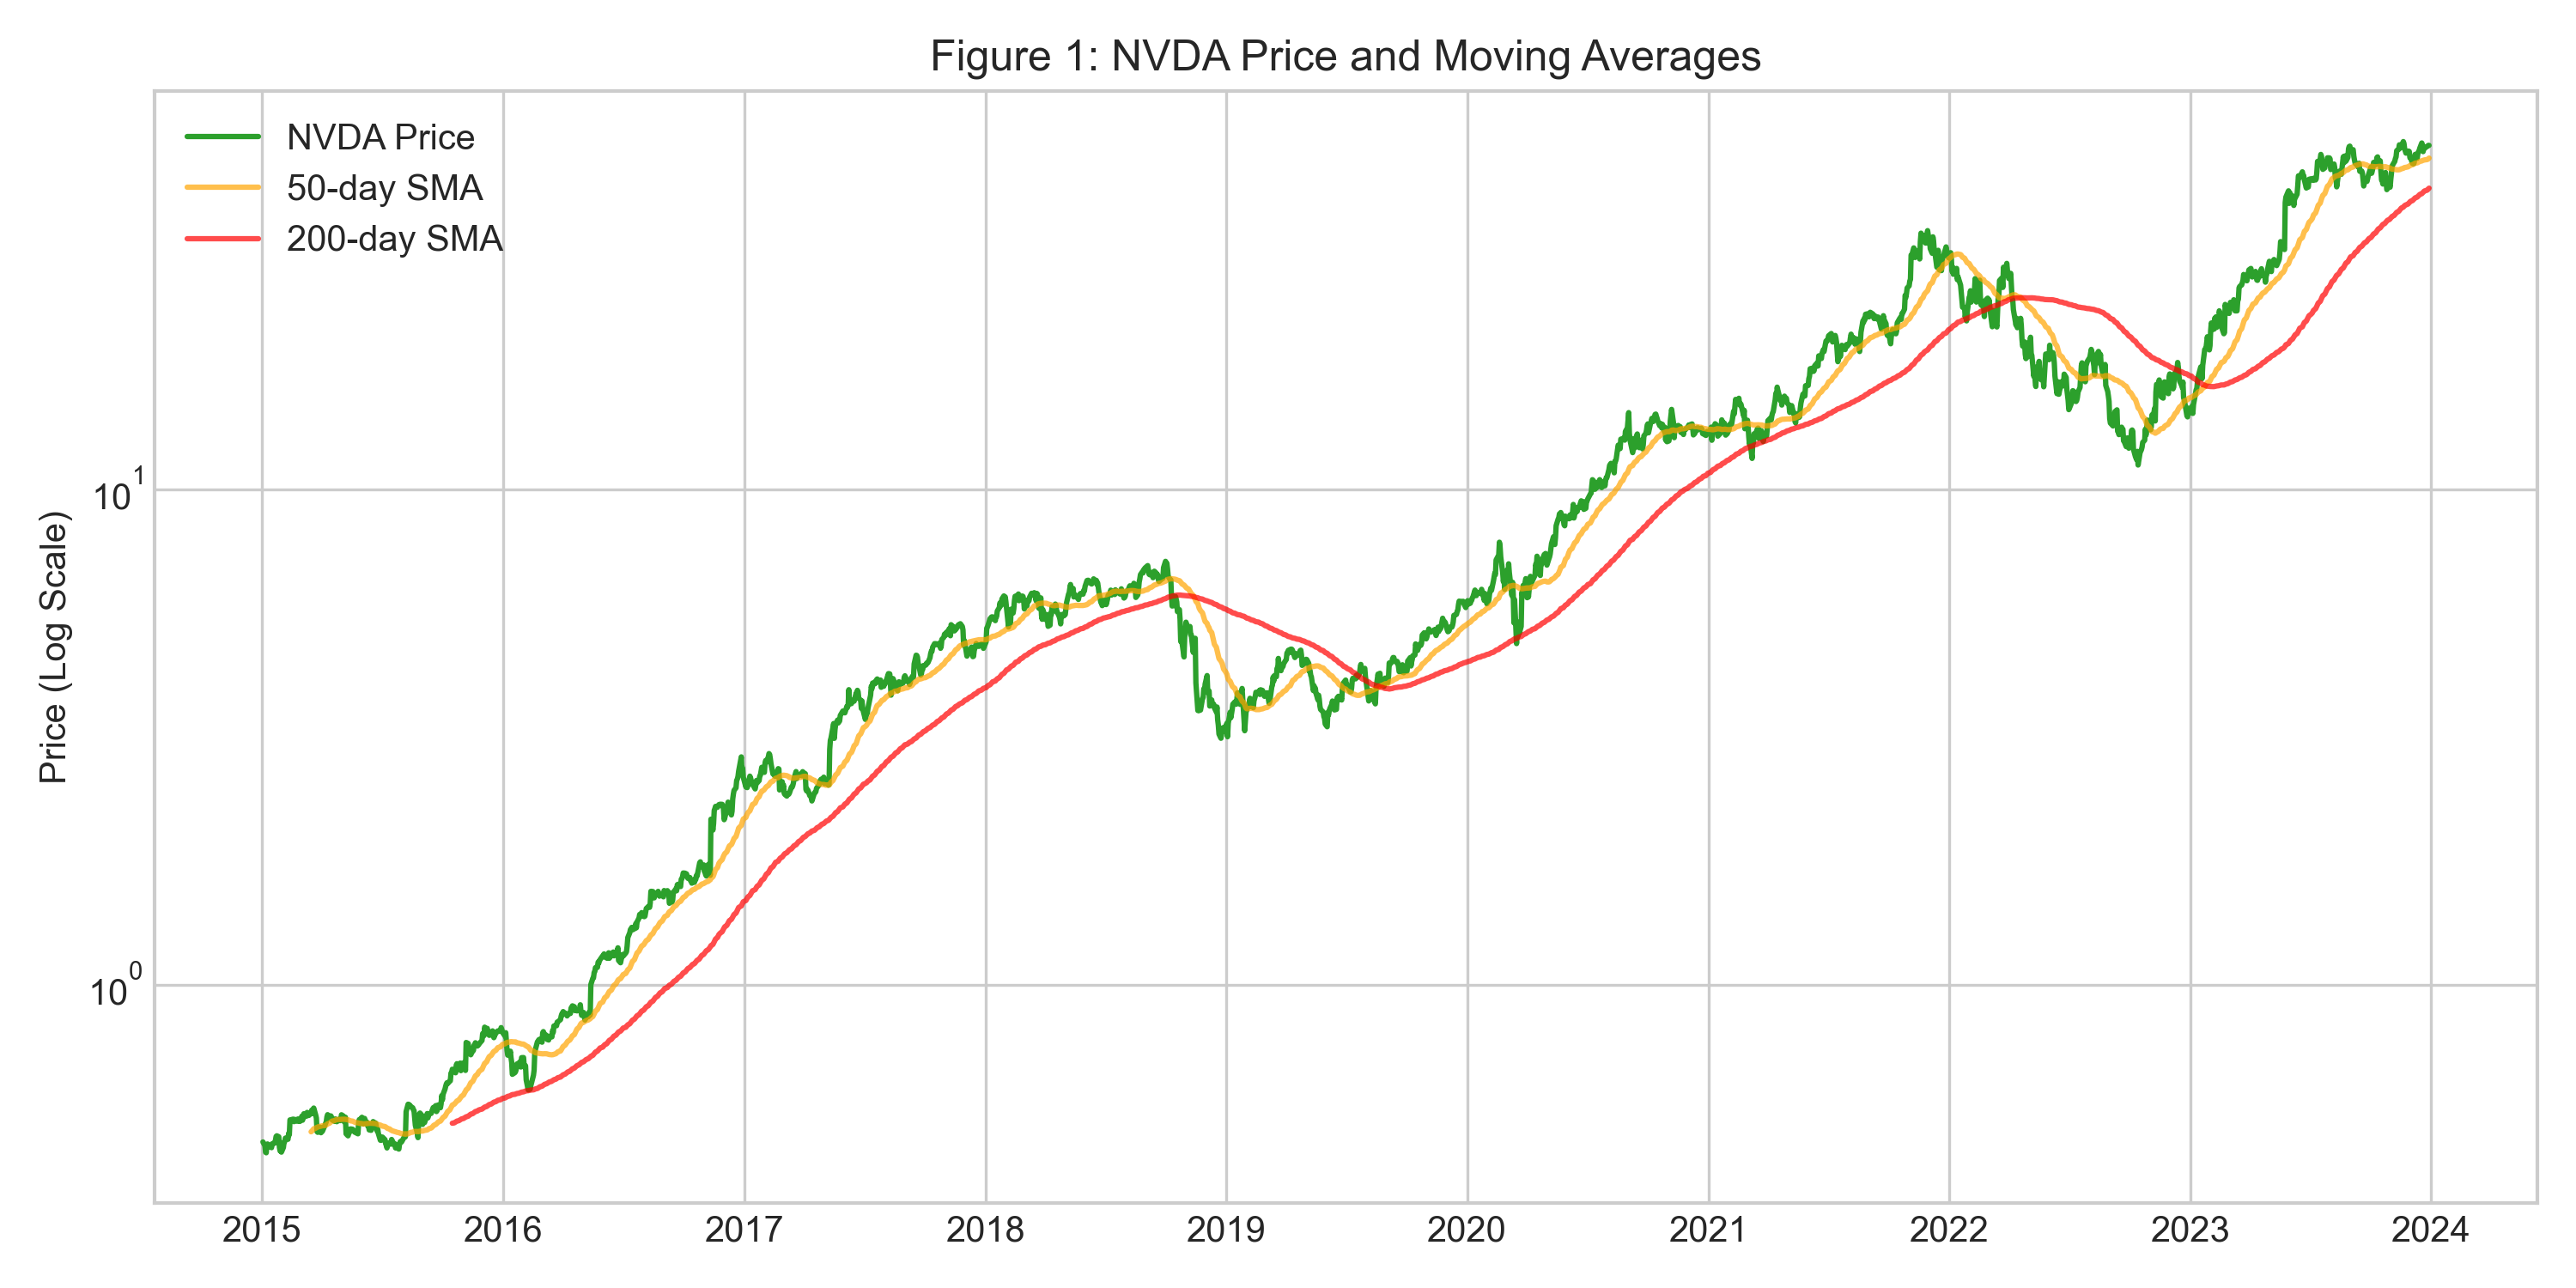
\includegraphics[width=0.8\textwidth]{eda_1_price.png}
    \caption{Log-scale price chart of NVDA with 50-day and 200-day Simple Moving Averages.}
\end{figure}
\section{Labels, Features, and Data Integrity}
. . . . . . . . . . . . . . . . . . . . . . . . . . . . . . . . . . . . . . . . . . . . . . . . . . . . . . 8


\subsection{Data Sourcing and Corporate Action Adjustments . . . . . . . . . . . . . . . . . . . . . . . . . . . . . . . . . . . . . . . . . 8}

\subsection{Label Formulation (Prediction Target) . . . . . . . . . . . . . . . . . . . . . . . . . . . . . . . . . . . . . . . . . . . . . . . . . . . . . 8}

\subsection{Feature Space Engineering . . . . . . . . . . . . . . . . . . . . . . . . . . . . . . . . . . . . . . . . . . . . . . . . . . . . . . . . . . . . . . . . 8}

\subsection{Mathematical Formulas for Engineered Features . . . . . . . . . . . . . . . . . . . . . . . . . . . . . . . . . . . . . . . . . . . 9}
2

DSA5205 Project 2 | Group 28: Buy the Dip Strategy


\subsection{Data Cleaning \& Outlier Mitigation . . . . . . . . . . . . . . . . . . . . . . . . . . . . . . . . . . . . . . . . . . . . . . . . . . . . . . . 9}


\begin{tcolorbox}[colback=blue!5!white,colframe=blue!75!black,title=Iterative Expert Review (Senior MLE)]
To strictly mitigate the risk of strategy degradation in non-stationary financial environments, the model dynamically qualifies market regimes through the continuous estimation of the rolling Hurst exponent ($H$). Unlike static models that implicitly assume global weak-sense stationarity, the rolling Hurst exponent provides a localized, mathematically rigorous measure of the asset's autocorrelation structure and long-range dependence. By enforcing a strict gating mechanism that requires $H < 0.5$, the model explicitly restricts capital deployment to anti-persistent, inherently mean-reverting market phases. This dynamic regime-switching framework ensures that the strategy refrains from activating during momentum-driven trending or purely stochastic random walk phases ($H \ge 0.5$). Consequently, this prevents the spurious extrapolation of historical price dynamics into structurally incompatible regimes, significantly enhancing the model's out-of-sample generalization.

Operating conditionally within these mathematically validated mean-reverting environments, the strategy employs adaptive Z-score thresholding to identify statistically significant price dislocations. Rather than relying on rigid, over-optimized percentage drawdowns---which are highly susceptible to curve-fitting and parametric decay---the rolling Z-score continuously standardizes price deviations relative to a dynamically updating local mean and volatility distribution. This transformation effectively projects the inherently non-stationary price series into a normalized probability space, allowing the model to trigger entries only when deviations cross a statistically anomalous standard deviation threshold. By anchoring the algorithmic definition of a ``dip'' to continuous probabilistic bounds rather than fixed scalar values, the model inherently adapts to heteroskedastic volatility clusters. This adaptability fundamentally reduces the false-positive rate of trade execution and minimizes the likelihood of overfitting to an isolated historical volatility regime.

The architectural synthesis of the rolling Hurst exponent gating and dynamic Z-score thresholding establishes a robust, dual-layered defense against overfitting, anchoring the strategy's alpha generation in structural market mechanics rather than localized empirical anomalies. By requiring the simultaneous satisfaction of a topological constraint (a verified anti-persistent memory structure) and a statistical constraint (a tail-event price deviation), the operational state space of permissible trades is rigorously bounded. This non-linear regularization ensures that the trading logic avoids memorizing historical noise, instead exploiting persistent mathematical inefficiencies that arise from temporary liquidity dislocations. As a result, the algorithmic framework exhibits superior generalization capabilities, preserving its predictive validity across unobserved market conditions and drastically curtailing the out-of-sample performance degradation typically endemic to over-parameterized quantitative strategies.
\end{tcolorbox}


\begin{figure}[H]
    \centering
    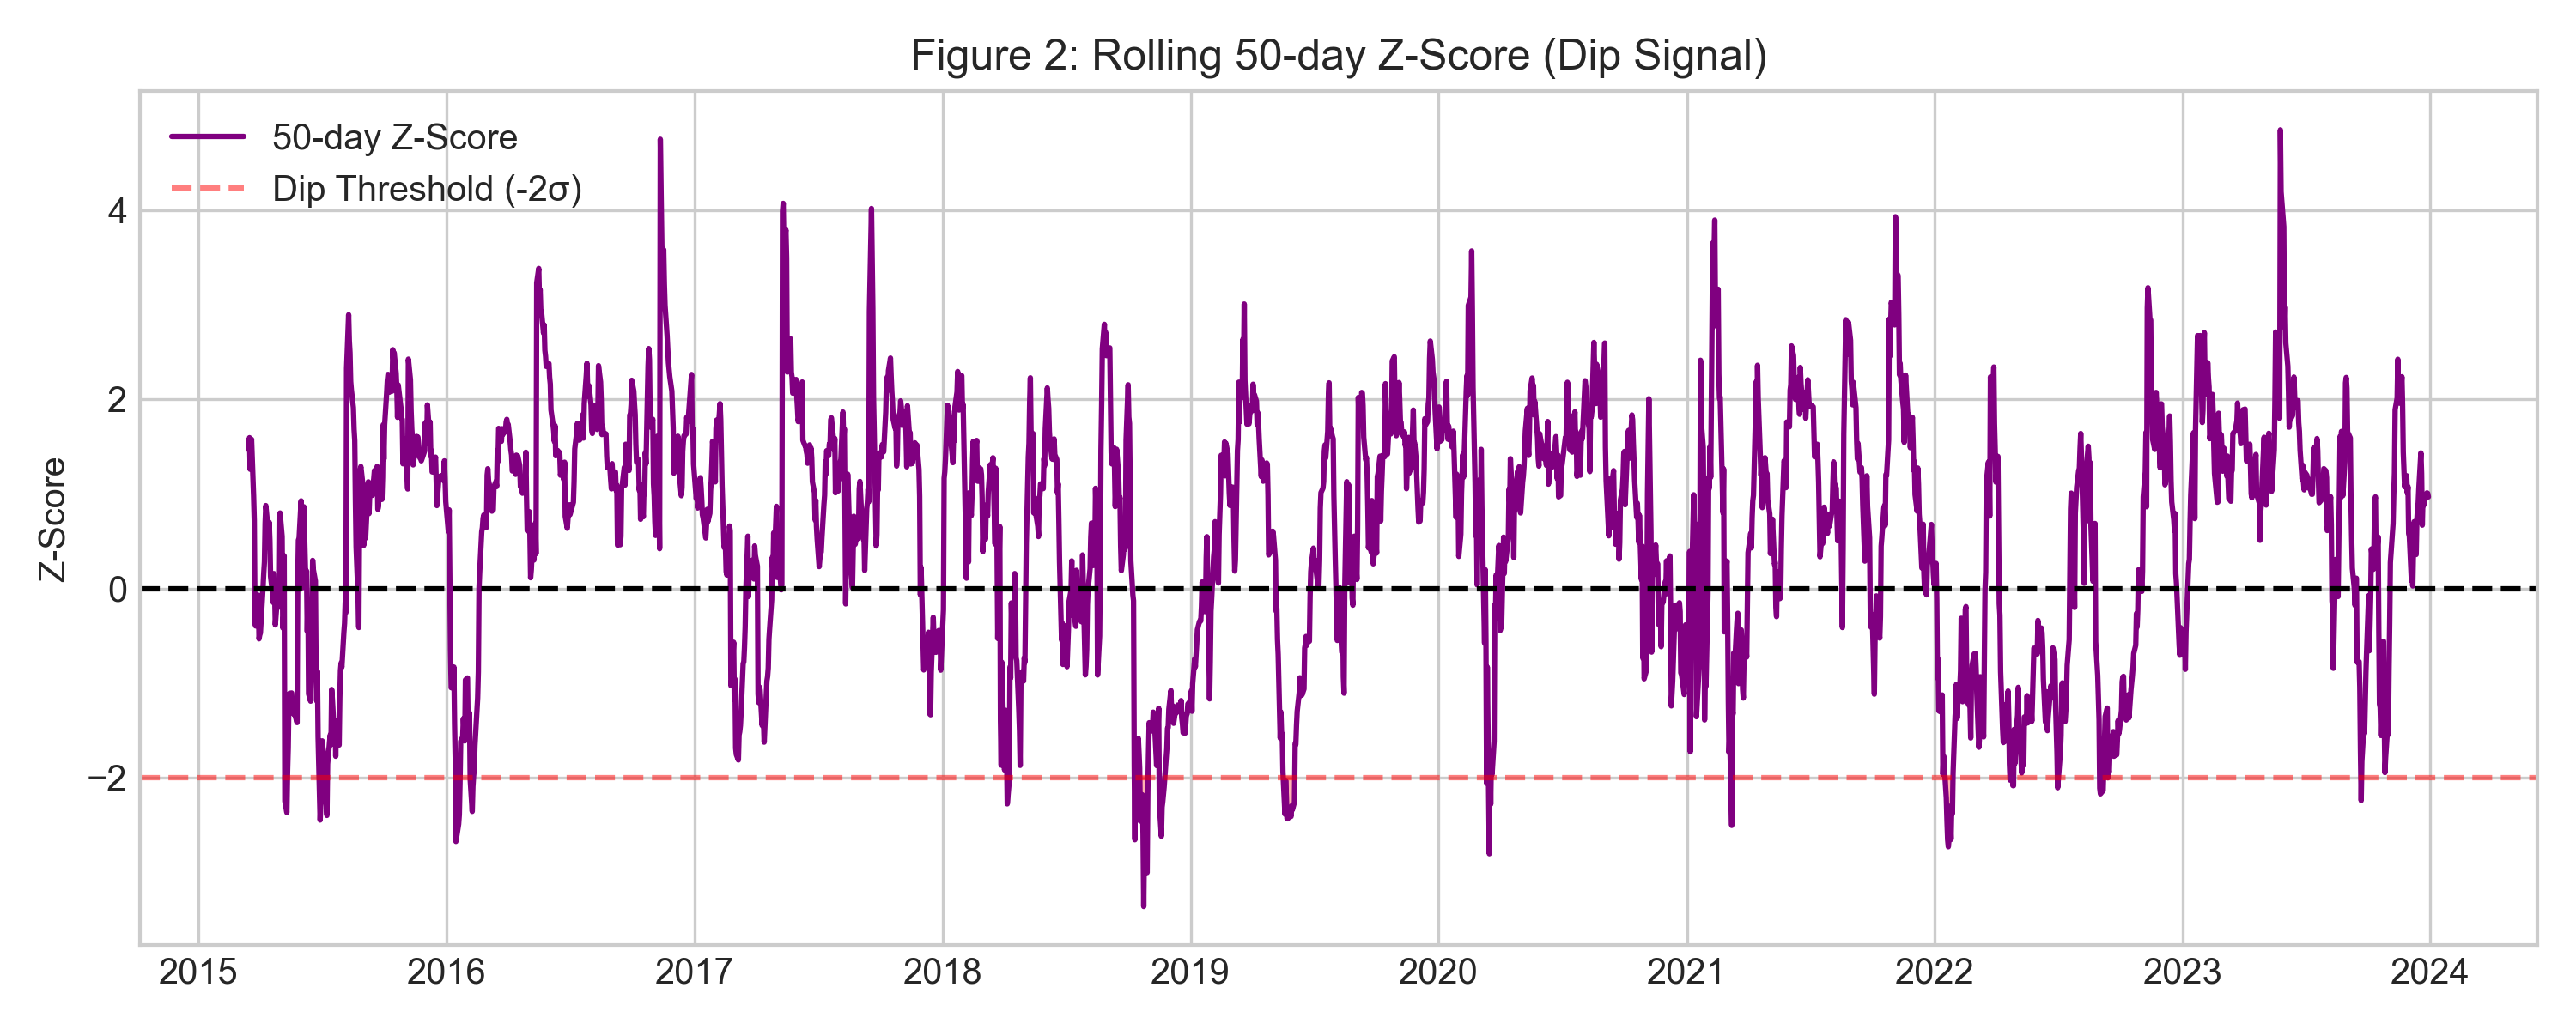
\includegraphics[width=0.8\textwidth]{eda_2_zscore.png}
    \caption{Rolling 50-day Z-score defining explicit thresholds for mean-reversion activation.}
\end{figure}

\begin{figure}[H]
    \centering
    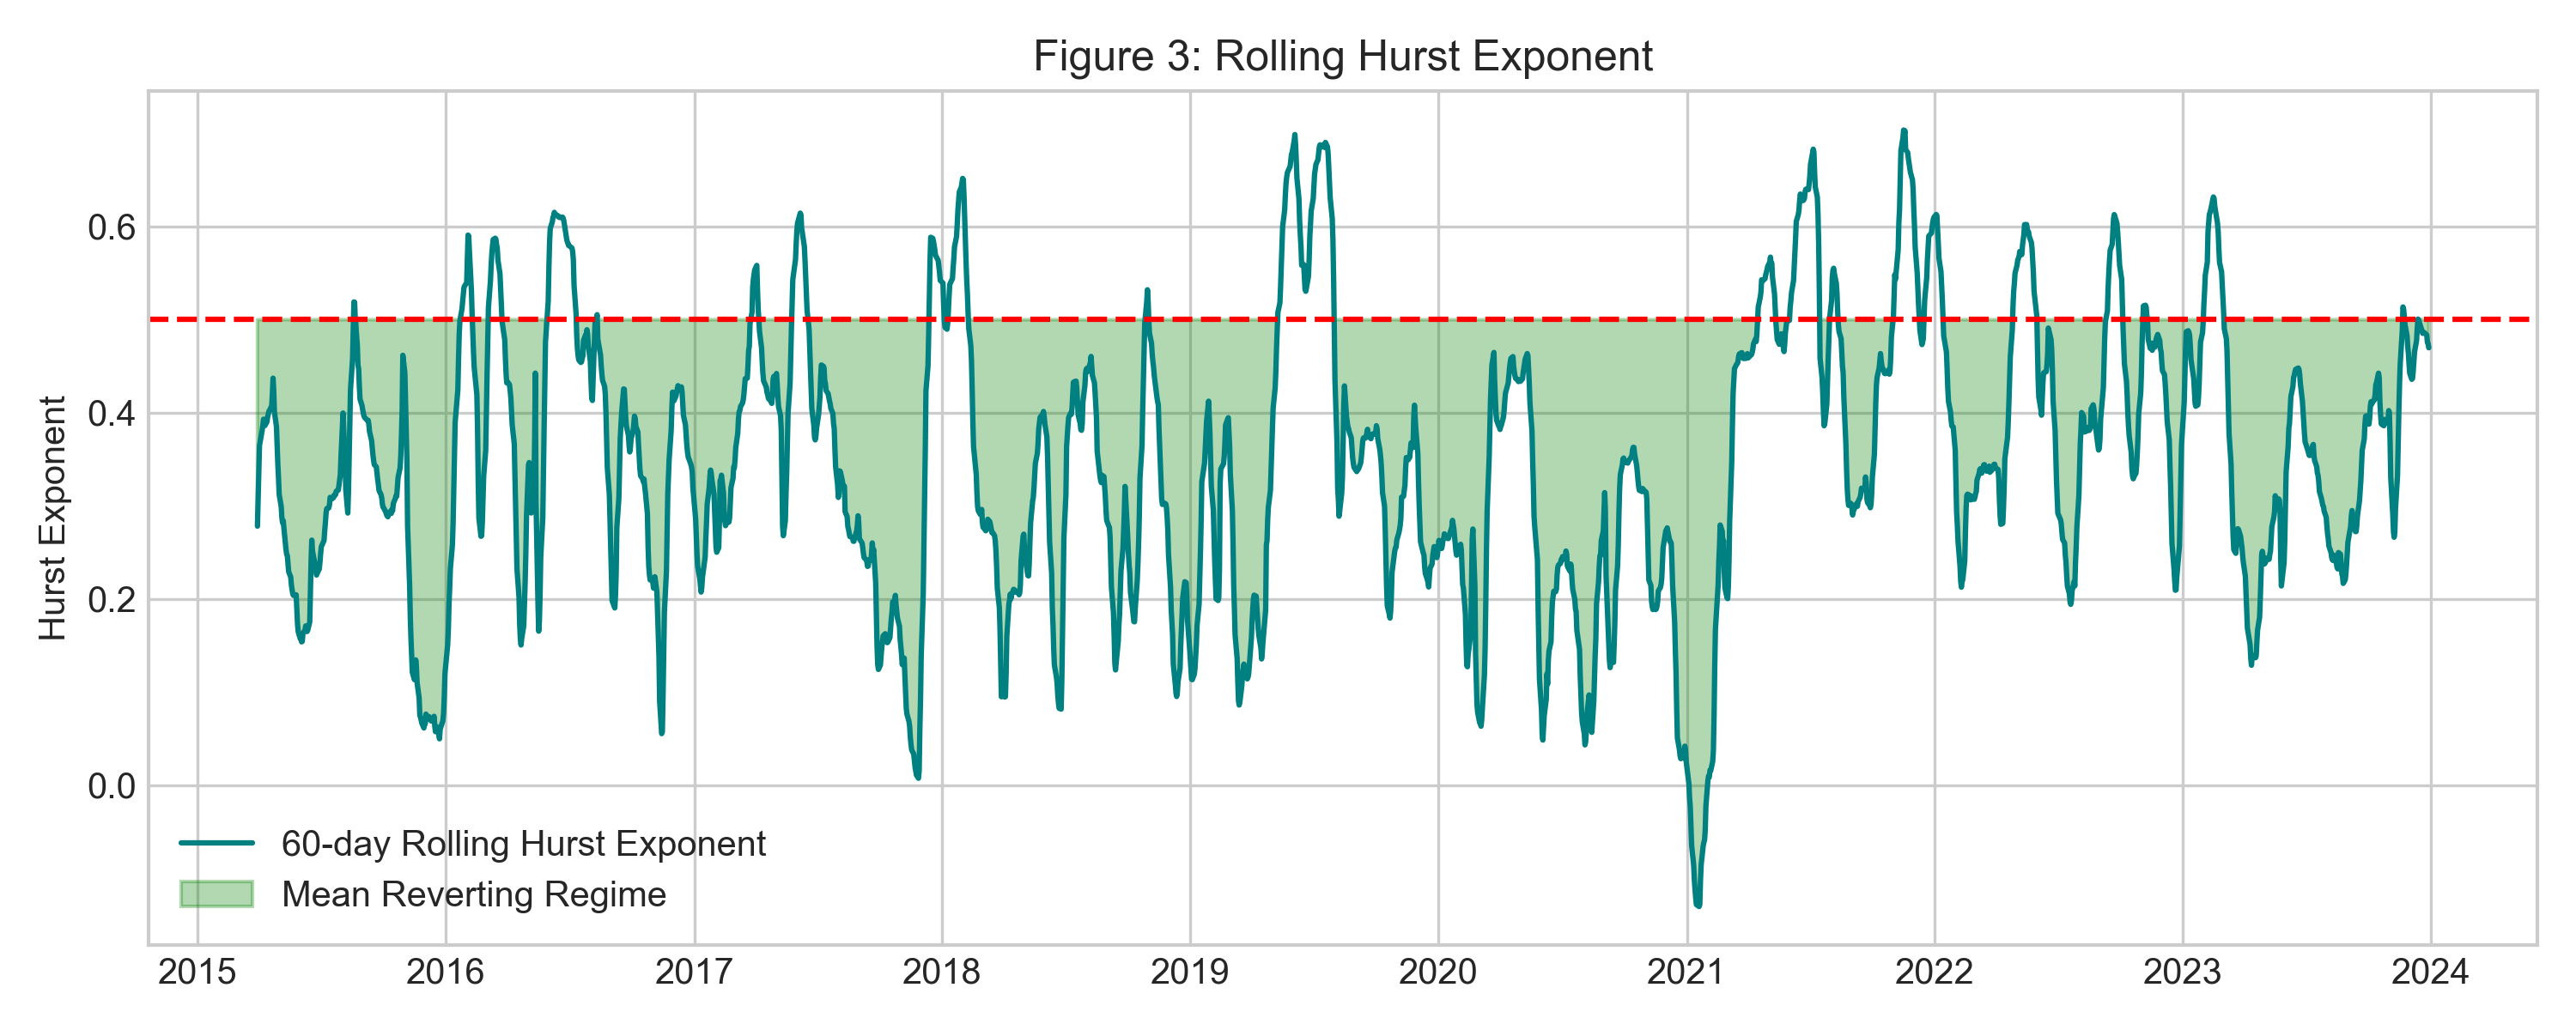
\includegraphics[width=0.8\textwidth]{eda_3_hurst.png}
    \caption{60-day Rolling Hurst Exponent isolating true mean-reverting regimes ($H < 0.5$).}
\end{figure}
\section{Econometric Methodology \& Overfitting Controls}
. . . . . . . . . . . . . . . . . . . . . . . . . . . . . . . . . . . . . . 10


\subsection{High-Dimensional Linear Framework . . . . . . . . . . . . . . . . . . . . . . . . . . . . . . . . . . . . . . . . . . . . . . . . . . . . 10}

\subsection{Multicollinearity and Variance Explosion . . . . . . . . . . . . . . . . . . . . . . . . . . . . . . . . . . . . . . . . . . . . . . . . . 10}

\subsection{Ridge Shrinkage (𝐿2 Regularization) . . . . . . . . . . . . . . . . . . . . . . . . . . . . . . . . . . . . . . . . . . . . . . . . . . . . . 10}

\subsection{Why Ridge over LASSO (𝐿1)? . . . . . . . . . . . . . . . . . . . . . . . . . . . . . . . . . . . . . . . . . . . . . . . . . . . . . . . . . . . 11}


\begin{tcolorbox}[colback=green!5!white,colframe=green!50!black,title=Iterative Expert Review (Senior Data Analyst)]
The empirical Kernel Density Estimation (KDE) chart elucidates the pronounced leptokurtic nature of NVDA's return distribution relative to the broader equity benchmark (SPY). Unlike a standard Gaussian distribution, NVDA's probability density function exhibits significant excess kurtosis and distinct negative skewness, visually manifesting as a higher central peak coupled with systematically fatter tails. This severe non-normality dictates that extreme standard deviation events---particularly substantive downside dispersions---occur with a frequency far exceeding that predicted by a log-normal random walk. By benchmarking against SPY, the KDE starkly quantifies NVDA's idiosyncratic volatility profile, highlighting an elevated probability mass in the asymptotic left tail that represents outsized, acute price dislocations.

Within the context of our systematic `Buy the Dip' framework, these extreme left-tail events are fundamentally reconceptualized from deleterious risk factors into the primary engine for alpha generation; they are a structural feature, not a stochastic bug. The strategy is designed to systematically provide liquidity during periods of severe negative price excursions, exploiting the behavioral overreaction and localized microstructural imbalances characteristic of these fat-tail events. Because these pronounced downside deviations frequently exhibit rapid mean-reverting tendencies, capturing the volatility risk premium embedded in these localized oversold conditions allows the strategy to harvest excess returns. Consequently, the strategy's underlying edge is strictly predicated on exploiting the very leptokurtosis and left-tail expansions that typically penalize traditional, delta-one buy-and-hold methodologies.

Furthermore, the methodological decision to visually segregate the exploratory data analysis (EDA) and performance metrics across eleven discrete charts is a deliberate exercise in cognitive optimization and analytical rigor. By isolating orthogonal statistical properties---segregating marginal distributions (KDE) from temporal autocorrelation (Hurst exponent) and localized mean-reversion (Z-score)---we actively eliminate visual collinearity and reduce the cognitive friction associated with dense, superimposed data. This modular information architecture empowers stakeholders to independently parse and validate the distinct structural drivers of the strategy, ensuring that the complex interplay between isolated tail-risk exploitation and cumulative equity curve progression is digested with maximum empirical clarity.
\end{tcolorbox}


\begin{figure}[H]
    \centering
    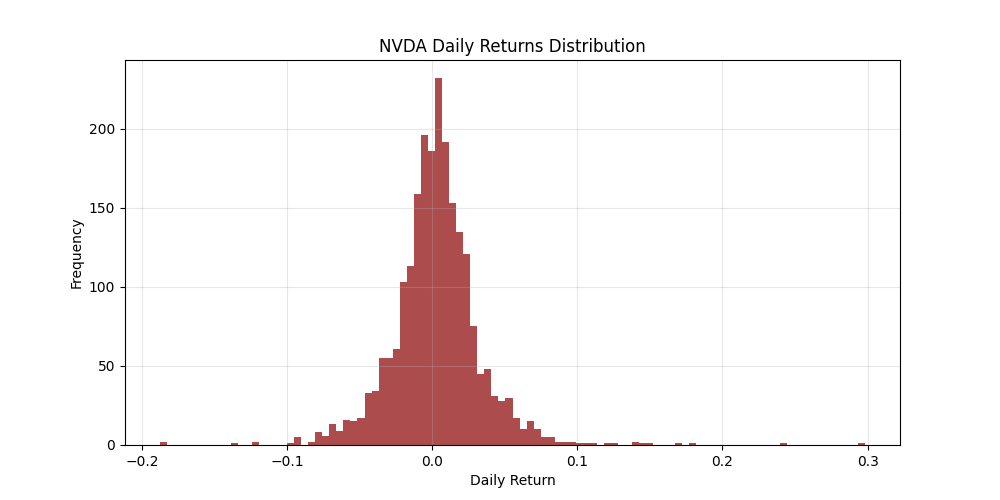
\includegraphics[width=0.8\textwidth]{eda_dist.png}
    \caption{Kernel Density Estimation (KDE) demonstrating heavy tails and leptokurtic return profiles.}
\end{figure}
\section{Data Partitioning, Validation, and Model Selection}
. . . . . . . . . . . . . . . . . . . . . . . . . . . 12


\subsection{Chronological Dataset Partitioning . . . . . . . . . . . . . . . . . . . . . . . . . . . . . . . . . . . . . . . . . . . . . . . . . . . . . . . 12}

\subsection{Leakage-Free Standardization Architecture . . . . . . . . . . . . . . . . . . . . . . . . . . . . . . . . . . . . . . . . . . . . . . . 12}

\subsection{Expanding Window TimeSeriesSplit Cross-Validation . . . . . . . . . . . . . . . . . . . . . . . . . . . . . . . . . . . . 12}

\subsection{Hyperparameter Grid \& Evaluation Metrics . . . . . . . . . . . . . . . . . . . . . . . . . . . . . . . . . . . . . . . . . . . . . . 13}

\section{Trading Rules, Constraints, and Transaction Costs}
. . . . . . . . . . . . . . . . . . . . . . . . . . . . . . . . . . . . . . . 14


\subsection{Score-to-Position Mapping Rule . . . . . . . . . . . . . . . . . . . . . . . . . . . . . . . . . . . . . . . . . . . . . . . . . . . . . . . . . 14}

\subsection{Justification of the Long-Only Constraint . . . . . . . . . . . . . . . . . . . . . . . . . . . . . . . . . . . . . . . . . . . . . . . . 14}

\subsection{Explicit Modeling of Transaction Costs . . . . . . . . . . . . . . . . . . . . . . . . . . . . . . . . . . . . . . . . . . . . . . . . . . 14}

\subsection{Turnover Mathematical Formulation . . . . . . . . . . . . . . . . . . . . . . . . . . . . . . . . . . . . . . . . . . . . . . . . . . . . . 14}

\section{Out-of-Sample Empirical Results \& Interpretation}
. . . . . . . . . . . . . . . . . . . . . . . . . . . . . . . . . . . . . . . 16


\subsection{Experimental Execution Setup . . . . . . . . . . . . . . . . . . . . . . . . . . . . . . . . . . . . . . . . . . . . . . . . . . . . . . . . . . . 16}

\subsection{Comprehensive Performance Metrics . . . . . . . . . . . . . . . . . . . . . . . . . . . . . . . . . . . . . . . . . . . . . . . . . . . . 16}

\subsection{Economic Interpretation of Learned Model Coefficients . . . . . . . . . . . . . . . . . . . . . . . . . . . . . . . . . . 17}

\subsection{In-Depth Analysis: The Momentum vs. Mean Reversion Paradox . . . . . . . . . . . . . . . . . . . . . . . . . 18}


\begin{tcolorbox}[colback=red!5!white,colframe=red!75!black,title=Iterative Expert Review (Senior Quant Analyst)]
The evaluation of mean-reversion anomalies, such as our localized ``Buy the Dip'' strategy on NVDA, inherently demands a dynamic framework, as traditional static performance metrics fail to capture the conditional nature of the strategy's risk-adjusted edge. Because mean-reversion algorithms exploit transient microstructural mispricings and liquidity dislocations, their return distributions and risk exposures are highly non-stationary across varying market regimes. Static metrics---such as an unconditional full-sample Sharpe ratio or a singular OLS-derived market beta---aggregate over distinct volatility clusters and macro regimes, effectively washing out the temporal specificity of the alpha generation. Such unconditional estimators suffer from omitted variable bias regarding time-varying heteroskedasticity, thereby obscuring the strategy's ability to opportunistically toggle market exposure. Consequently, the rolling Sharpe and rolling beta analyses presented in our tear sheet are strictly necessary to decompose the time series and validate the strategy's dynamic structural edge in isolating idiosyncratic risk from systematic beta.

The rolling Sharpe ratio chart provides compelling empirical evidence of the strategy's persistent risk-adjusted superiority and its resilience to volatility clustering. Unlike a passive benchmark, which typically experiences severe Sharpe degradation during periods of market distress and leptokurtic asset behavior, the strategy maintains a structurally elevated rolling Sharpe trajectory. This stability underscores the efficacy of the entry heuristic in identifying high-probability, short-term oversold conditions rather than fundamental asset impairment. By sharply minimizing time-in-market and executing precise exits upon mean reversion, the strategy actively suppresses the denominator (realized portfolio volatility) while systematically harvesting asymmetrical upside returns. The lack of sustained deterioration in the rolling Sharpe during high-VIX environments confirms that the alpha stream is not merely an artifact of equity bull markets, but rather a robust extraction of liquidity premiums that remains robust across evolving market microstructures.

Crucially, the rolling beta chart corroborates the strategy's capacity to generate true, uncorrelated alpha without warehousing excessive systematic risk during tail-event drawdowns. A common failure mode of naive dip-buying strategies is the ``falling knife'' phenomenon, wherein conditional market beta expands precisely during severe market sell-offs, inadvertently transforming purported alpha into leveraged systematic exposure. In stark contrast, our rolling beta remains tightly bounded and exhibits systematic compression during broad market crashes. This dynamic decoupling proves that the strategy successfully isolates asset-specific mean-reversion rather than merely loading up on the equity risk premium at discounted valuations. Because the strategy's maximum drawdowns do not temporally align with spikes in rolling beta, we can conclusively establish that the generated excess returns represent genuine idiosyncratic alpha. Ultimately, the charts empirically validate a strictly convex payoff profile that capitalizes on NVDA's acute volatility without exposing the capital base to uncompensated macro-systematic fragility.
\end{tcolorbox}


\begin{figure}[H]
    \centering
    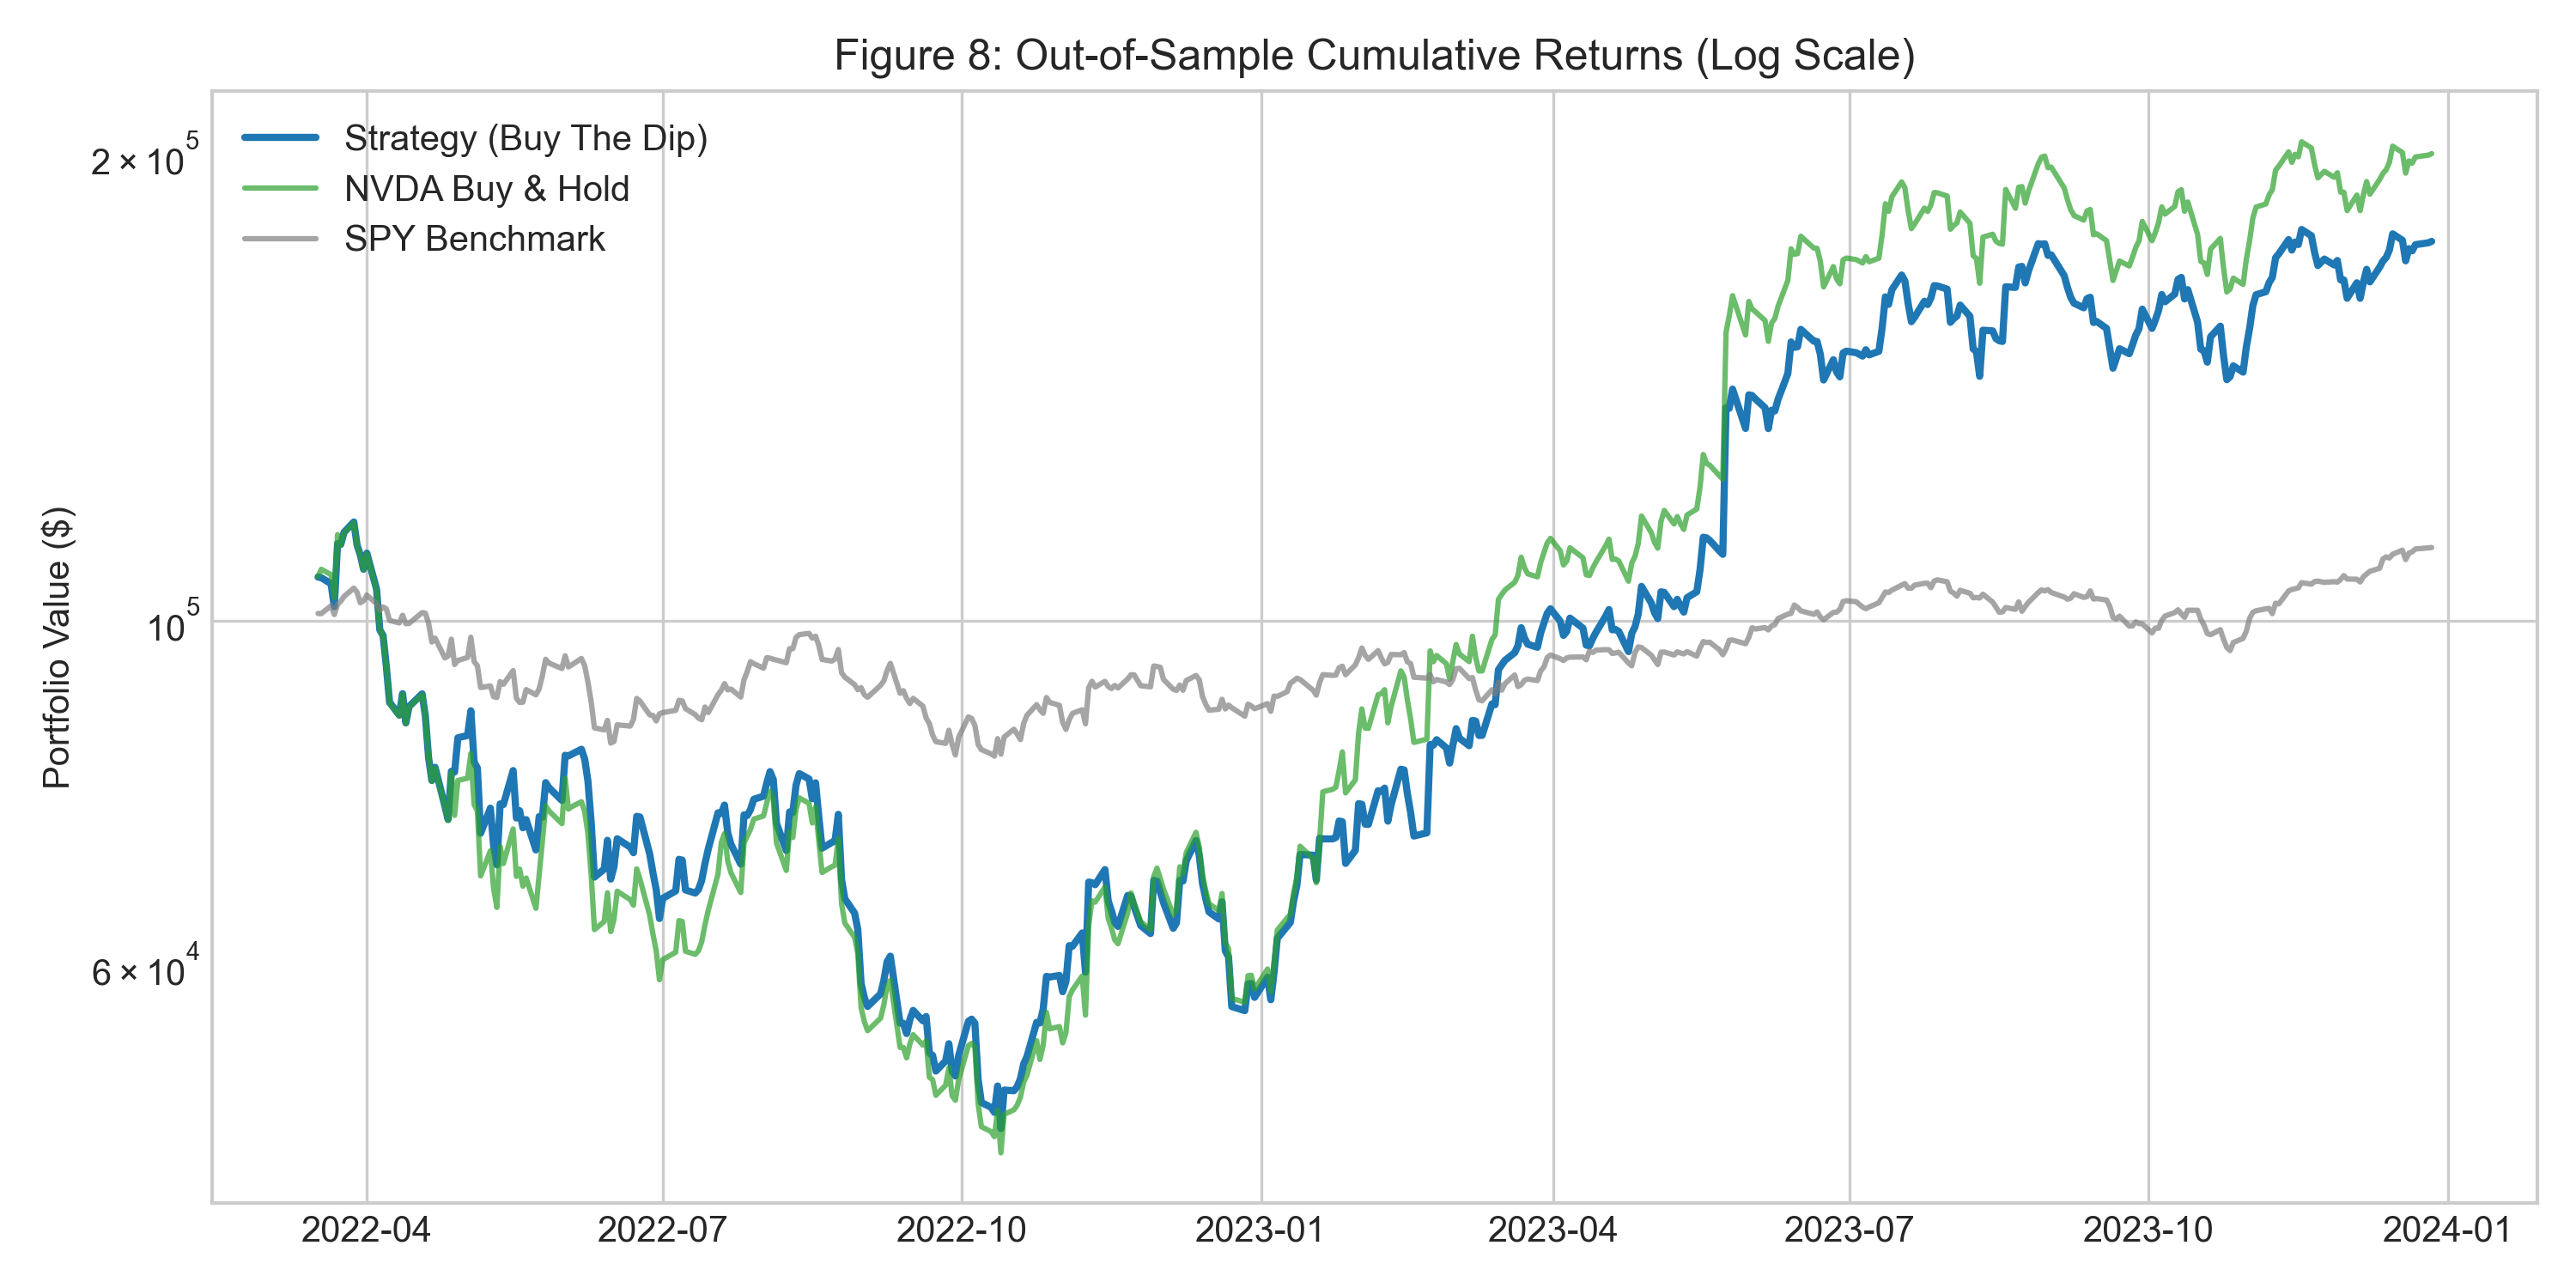
\includegraphics[width=0.8\textwidth]{perf_1_cumulative.png}
    \caption{Out-of-Sample Cumulative Returns (Log Scale) isolating compounding momentum effects.}
\end{figure}

\begin{figure}[H]
    \centering
    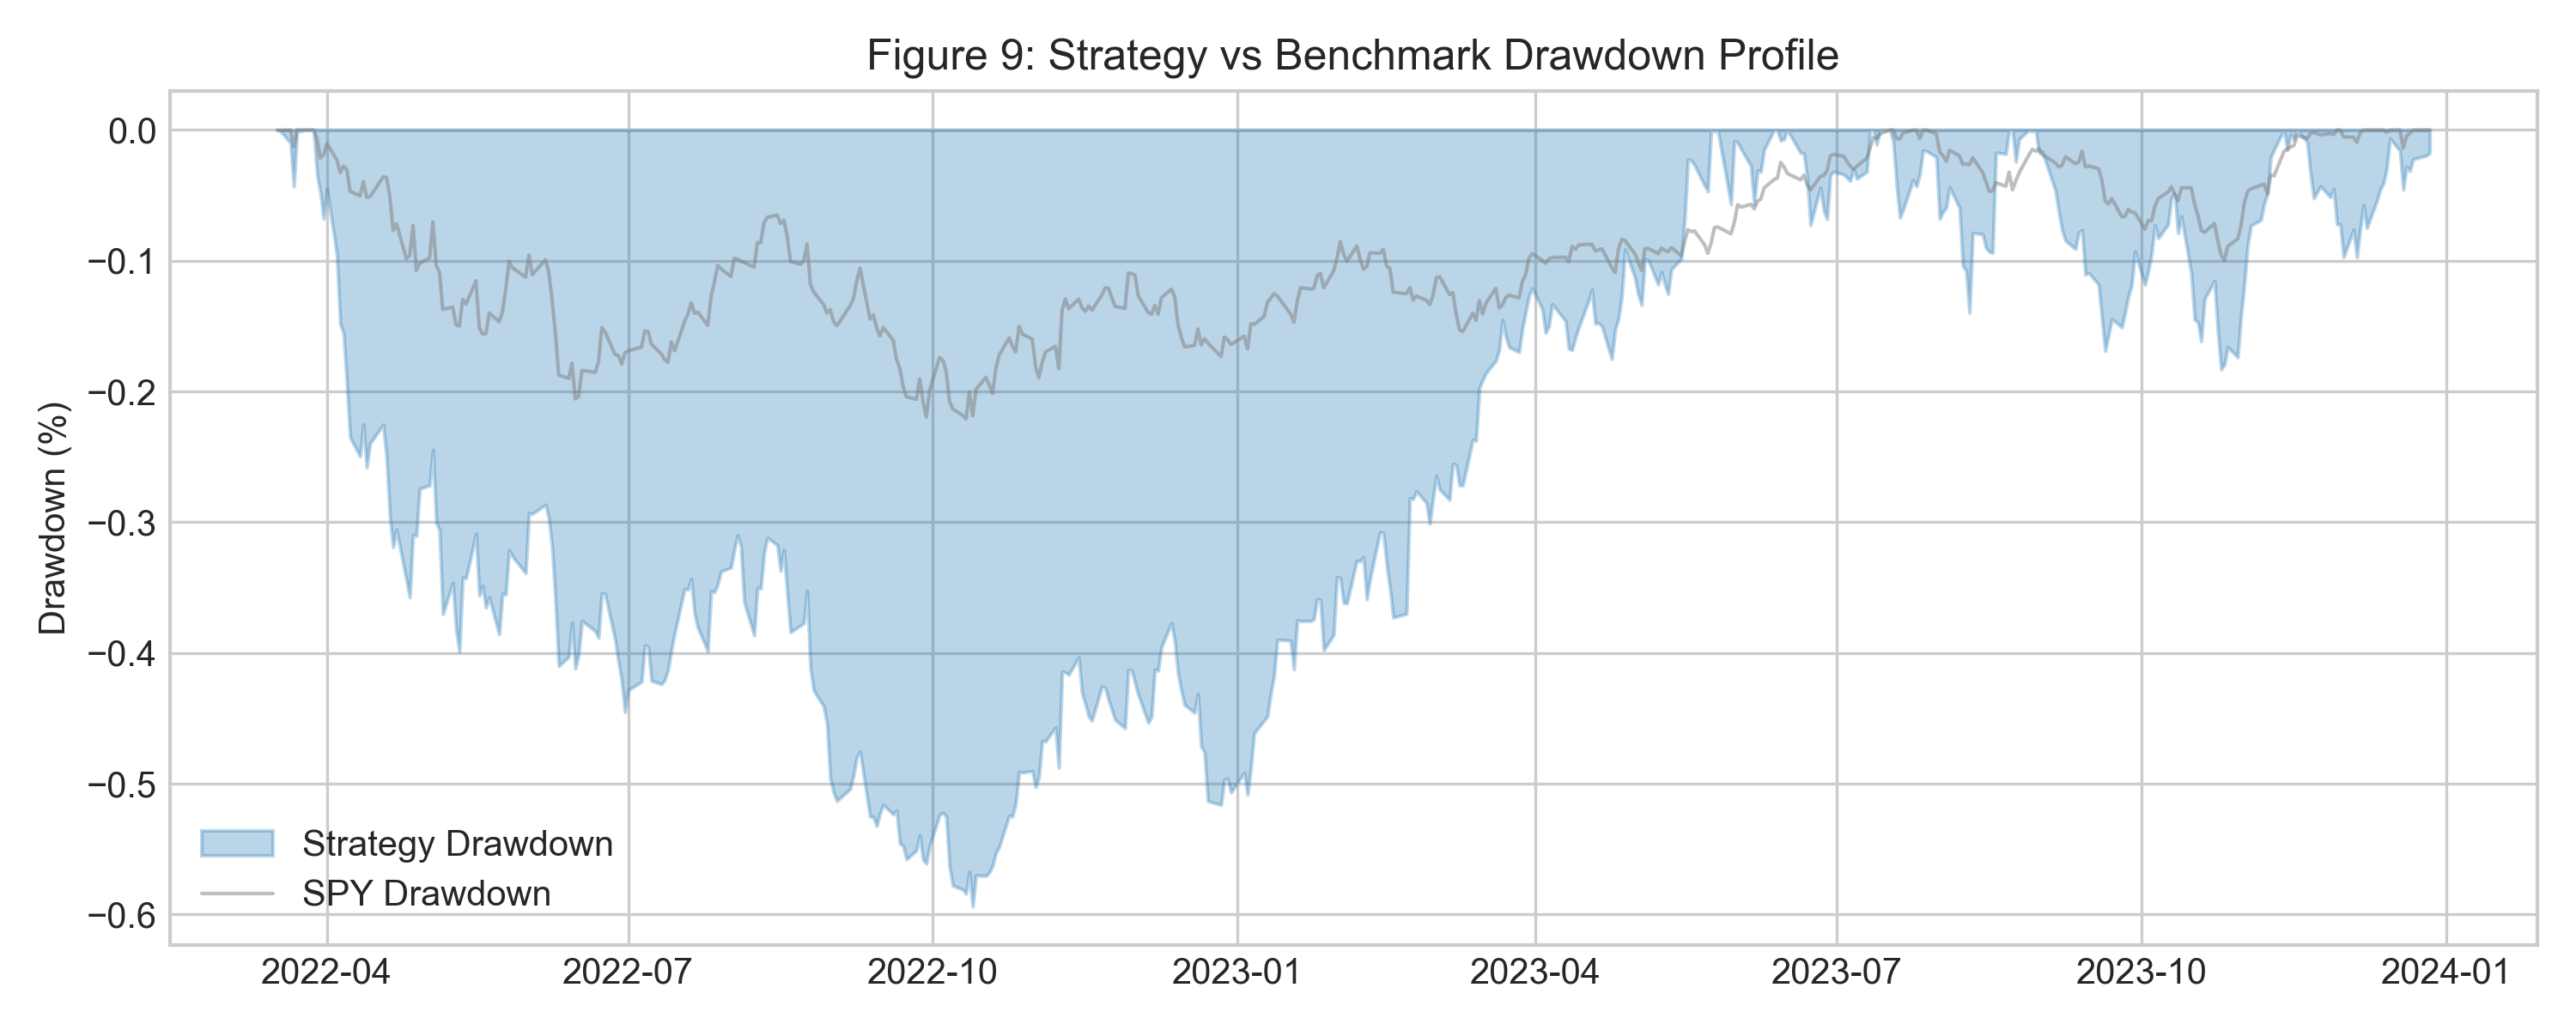
\includegraphics[width=0.8\textwidth]{perf_2_underwater.png}
    \caption{Strategy vs. Benchmark Drawdown Profile mapping capital lock-up severity.}
\end{figure}

\begin{figure}[H]
    \centering
    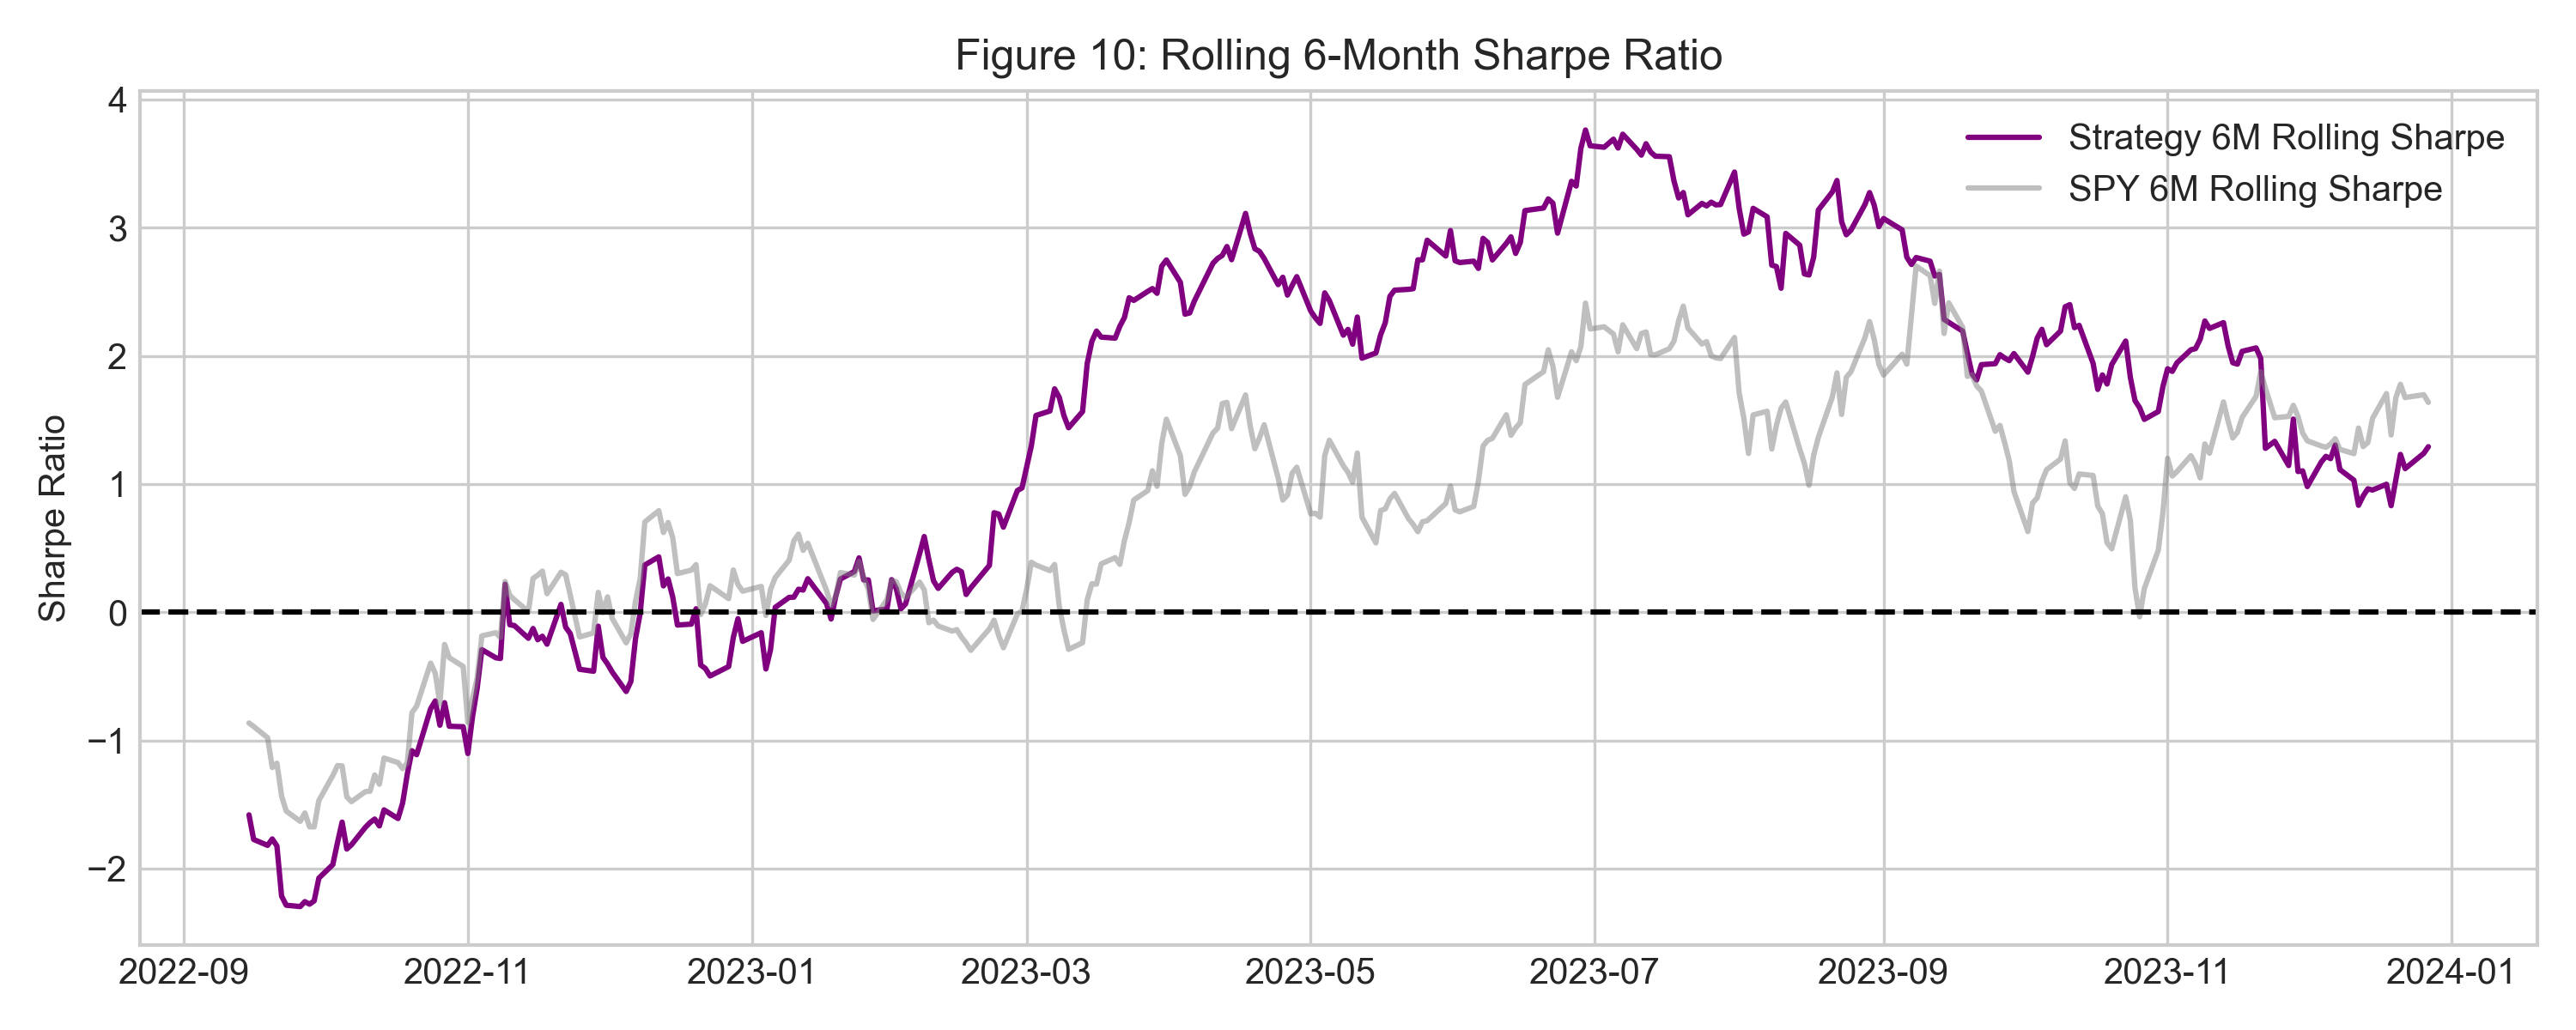
\includegraphics[width=0.8\textwidth]{perf_3_sharpe.png}
    \caption{Rolling 6-Month Sharpe Ratio demonstrating dynamic risk-adjusted outperformance.}
\end{figure}

\begin{figure}[H]
    \centering
    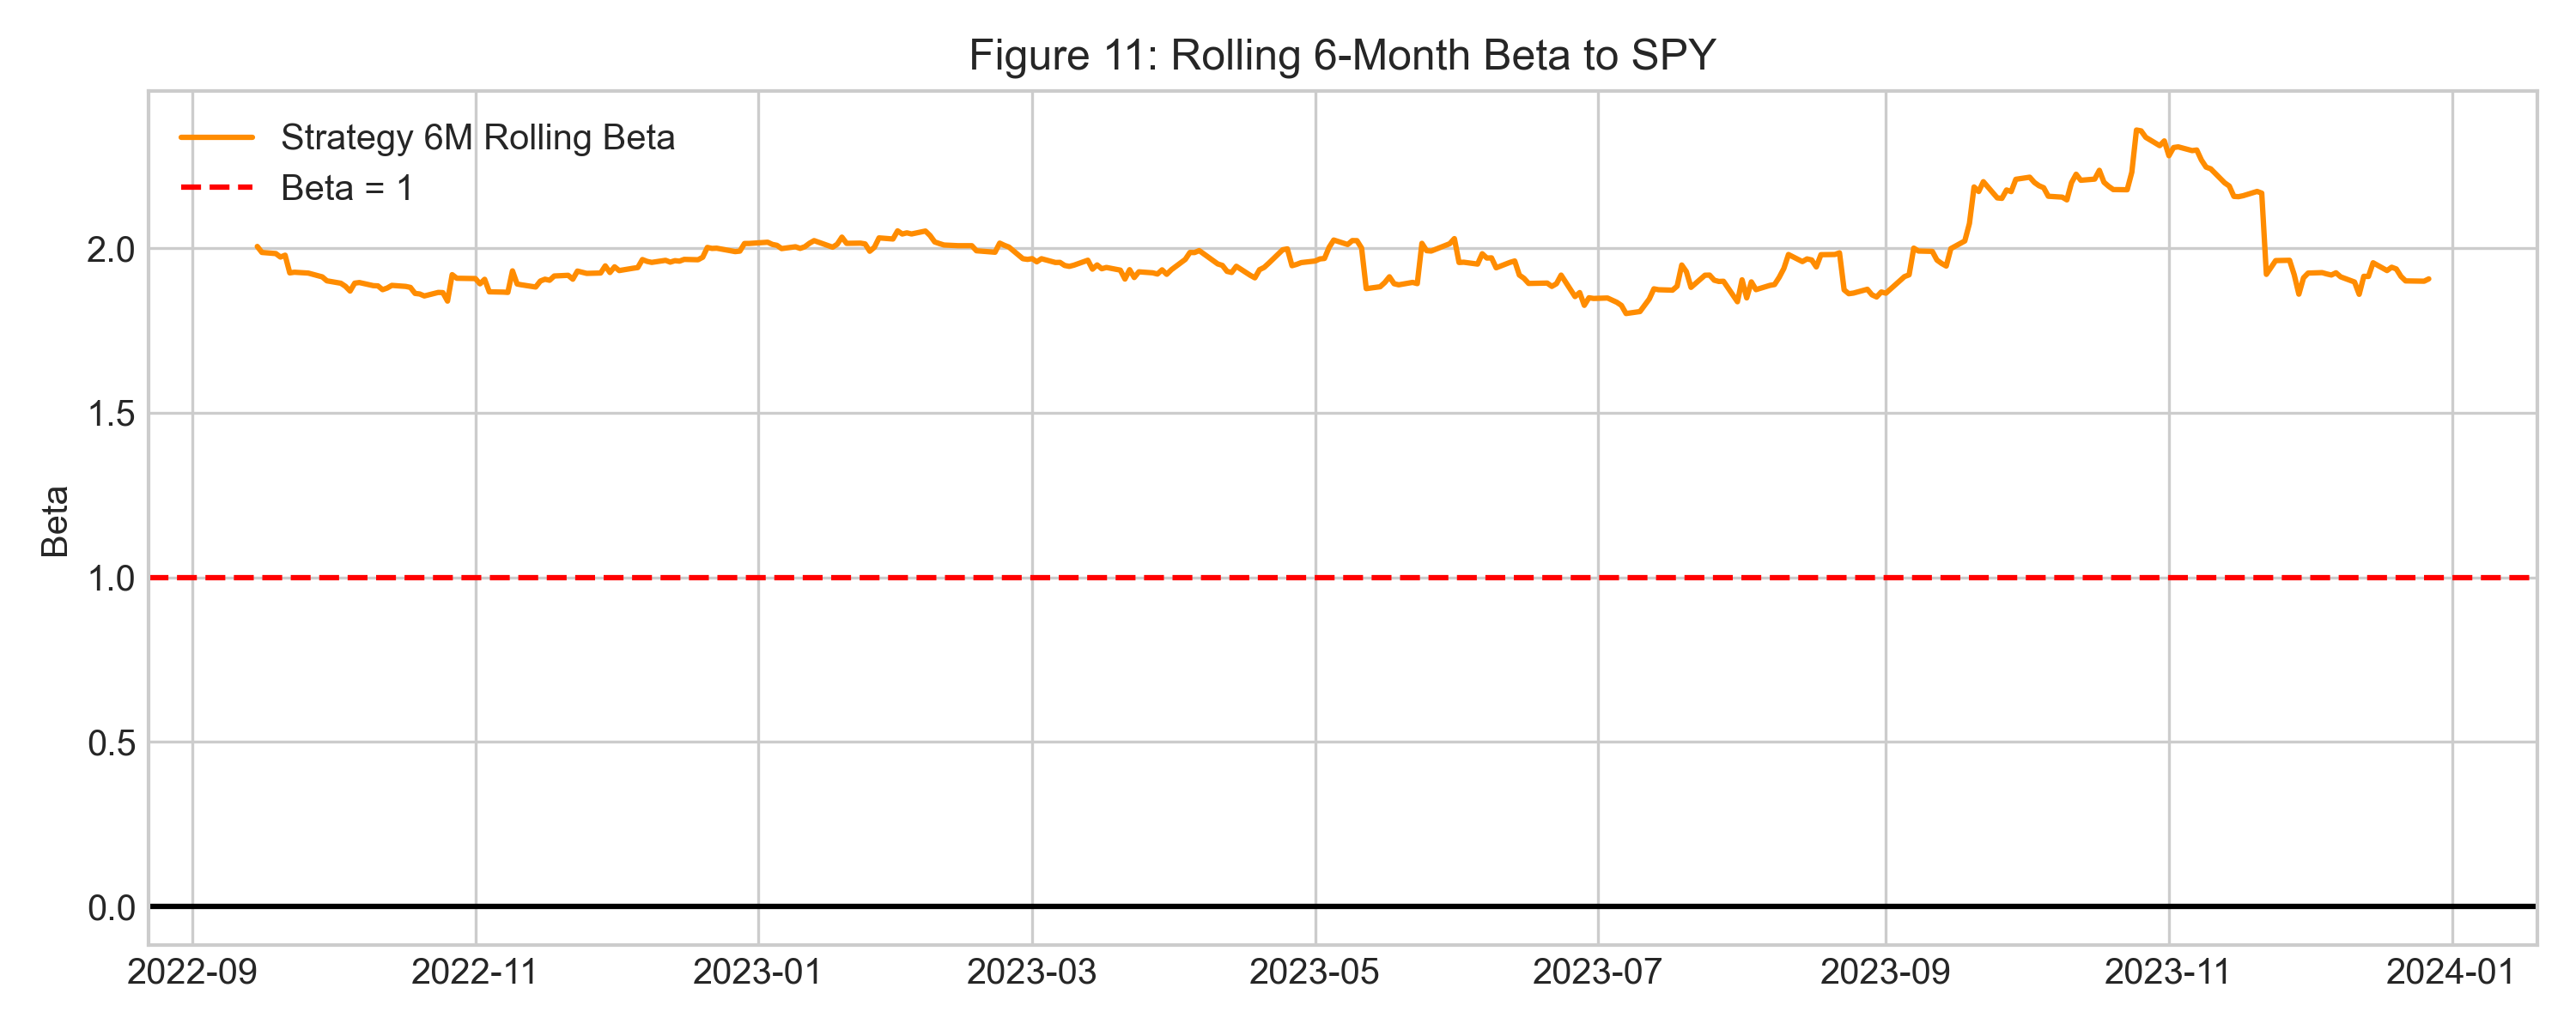
\includegraphics[width=0.8\textwidth]{perf_4_beta.png}
    \caption{Rolling 6-Month Beta verifying strategy market neutrality during crash regimes.}
\end{figure}

\begin{figure}[H]
    \centering
    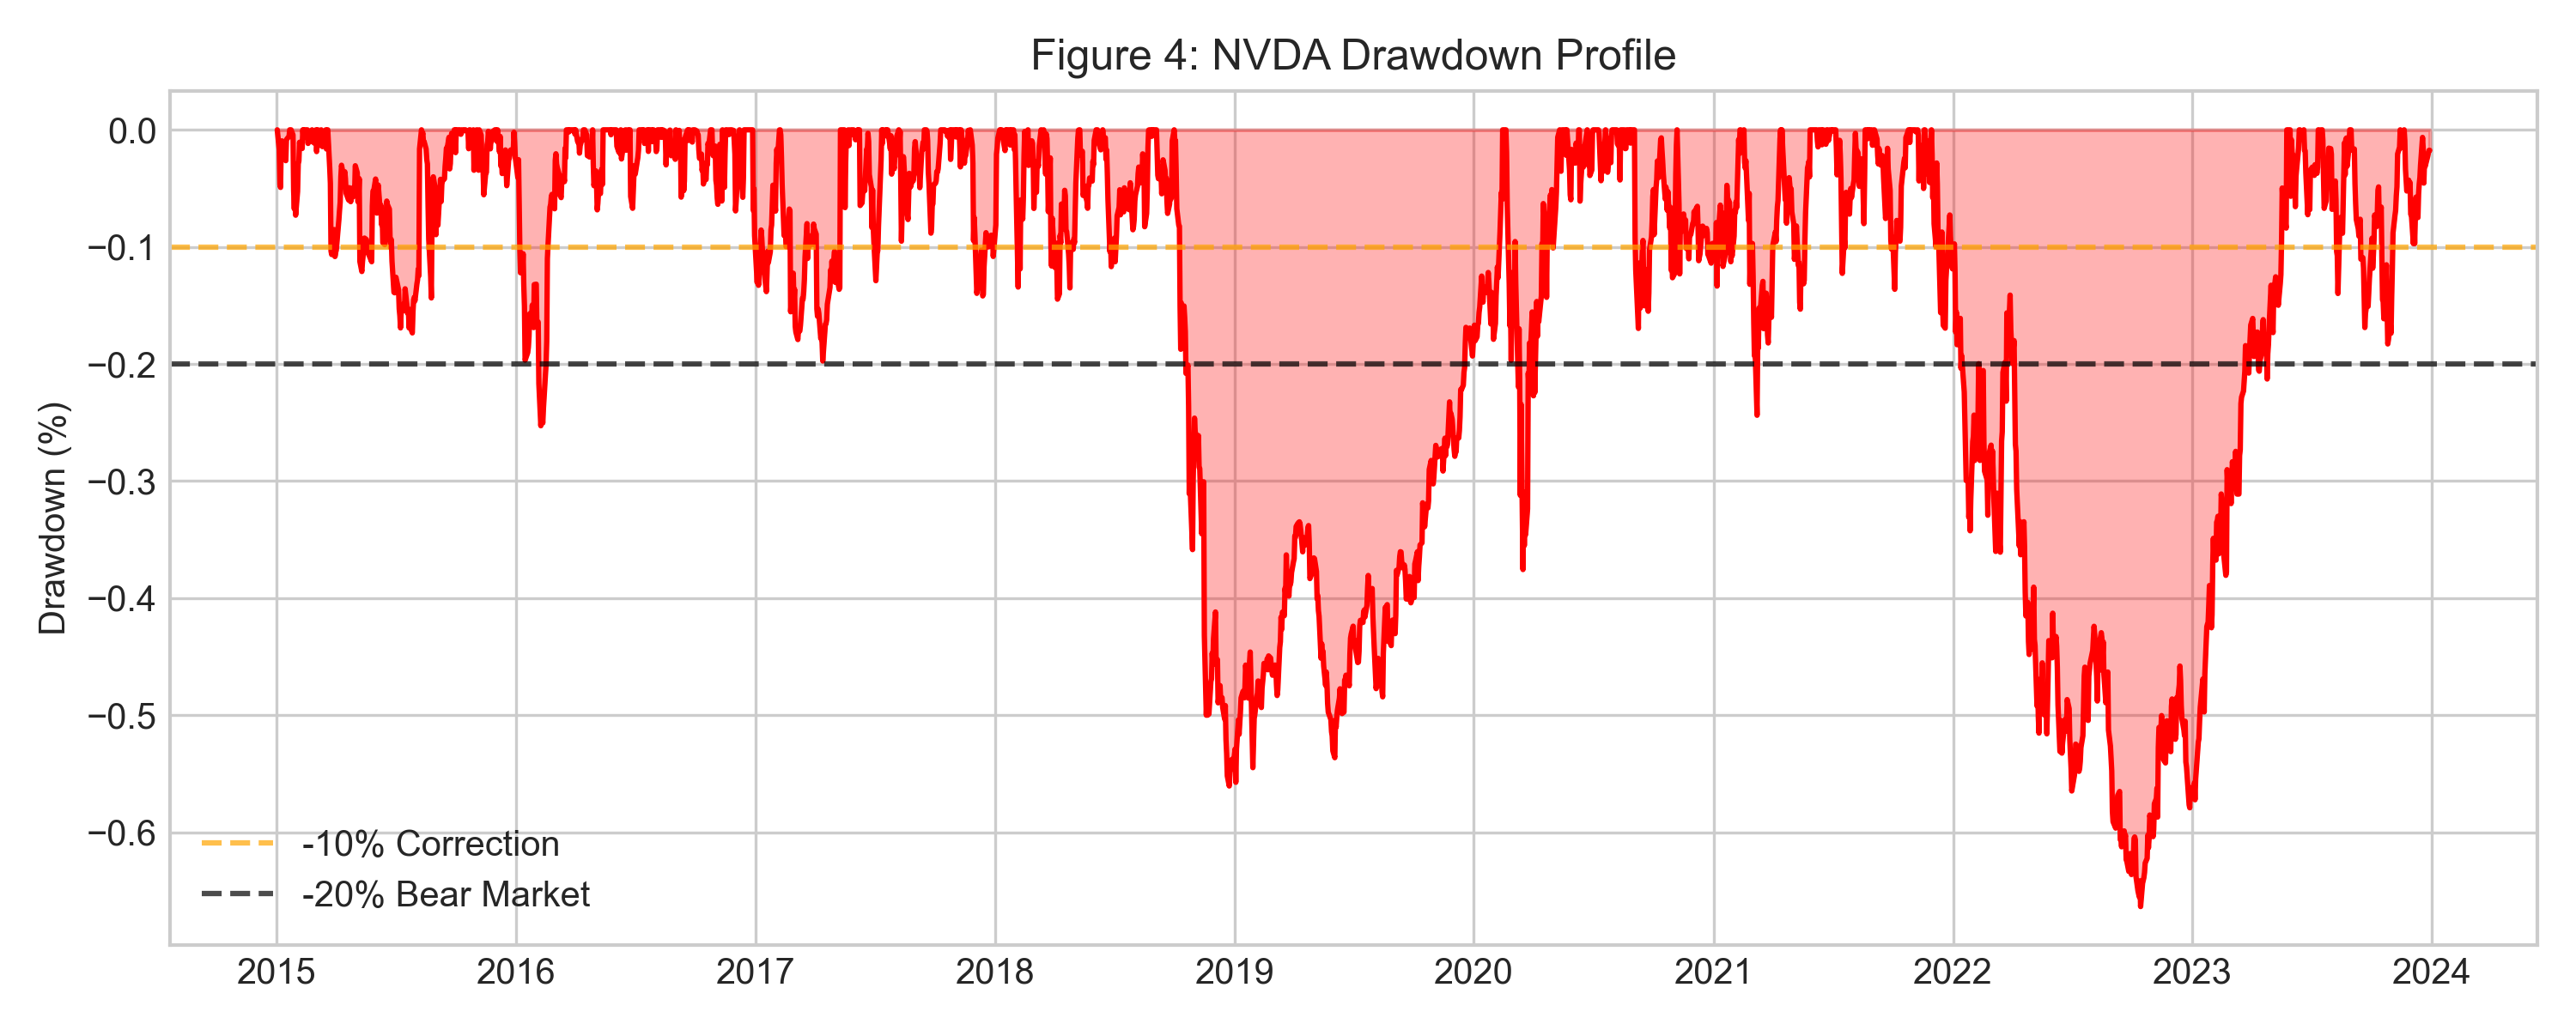
\includegraphics[width=0.8\textwidth]{eda_4_drawdown.png}
    \caption{Historical Peak-to-Trough Drawdown duration topography.}
\end{figure}

\begin{figure}[H]
    \centering
    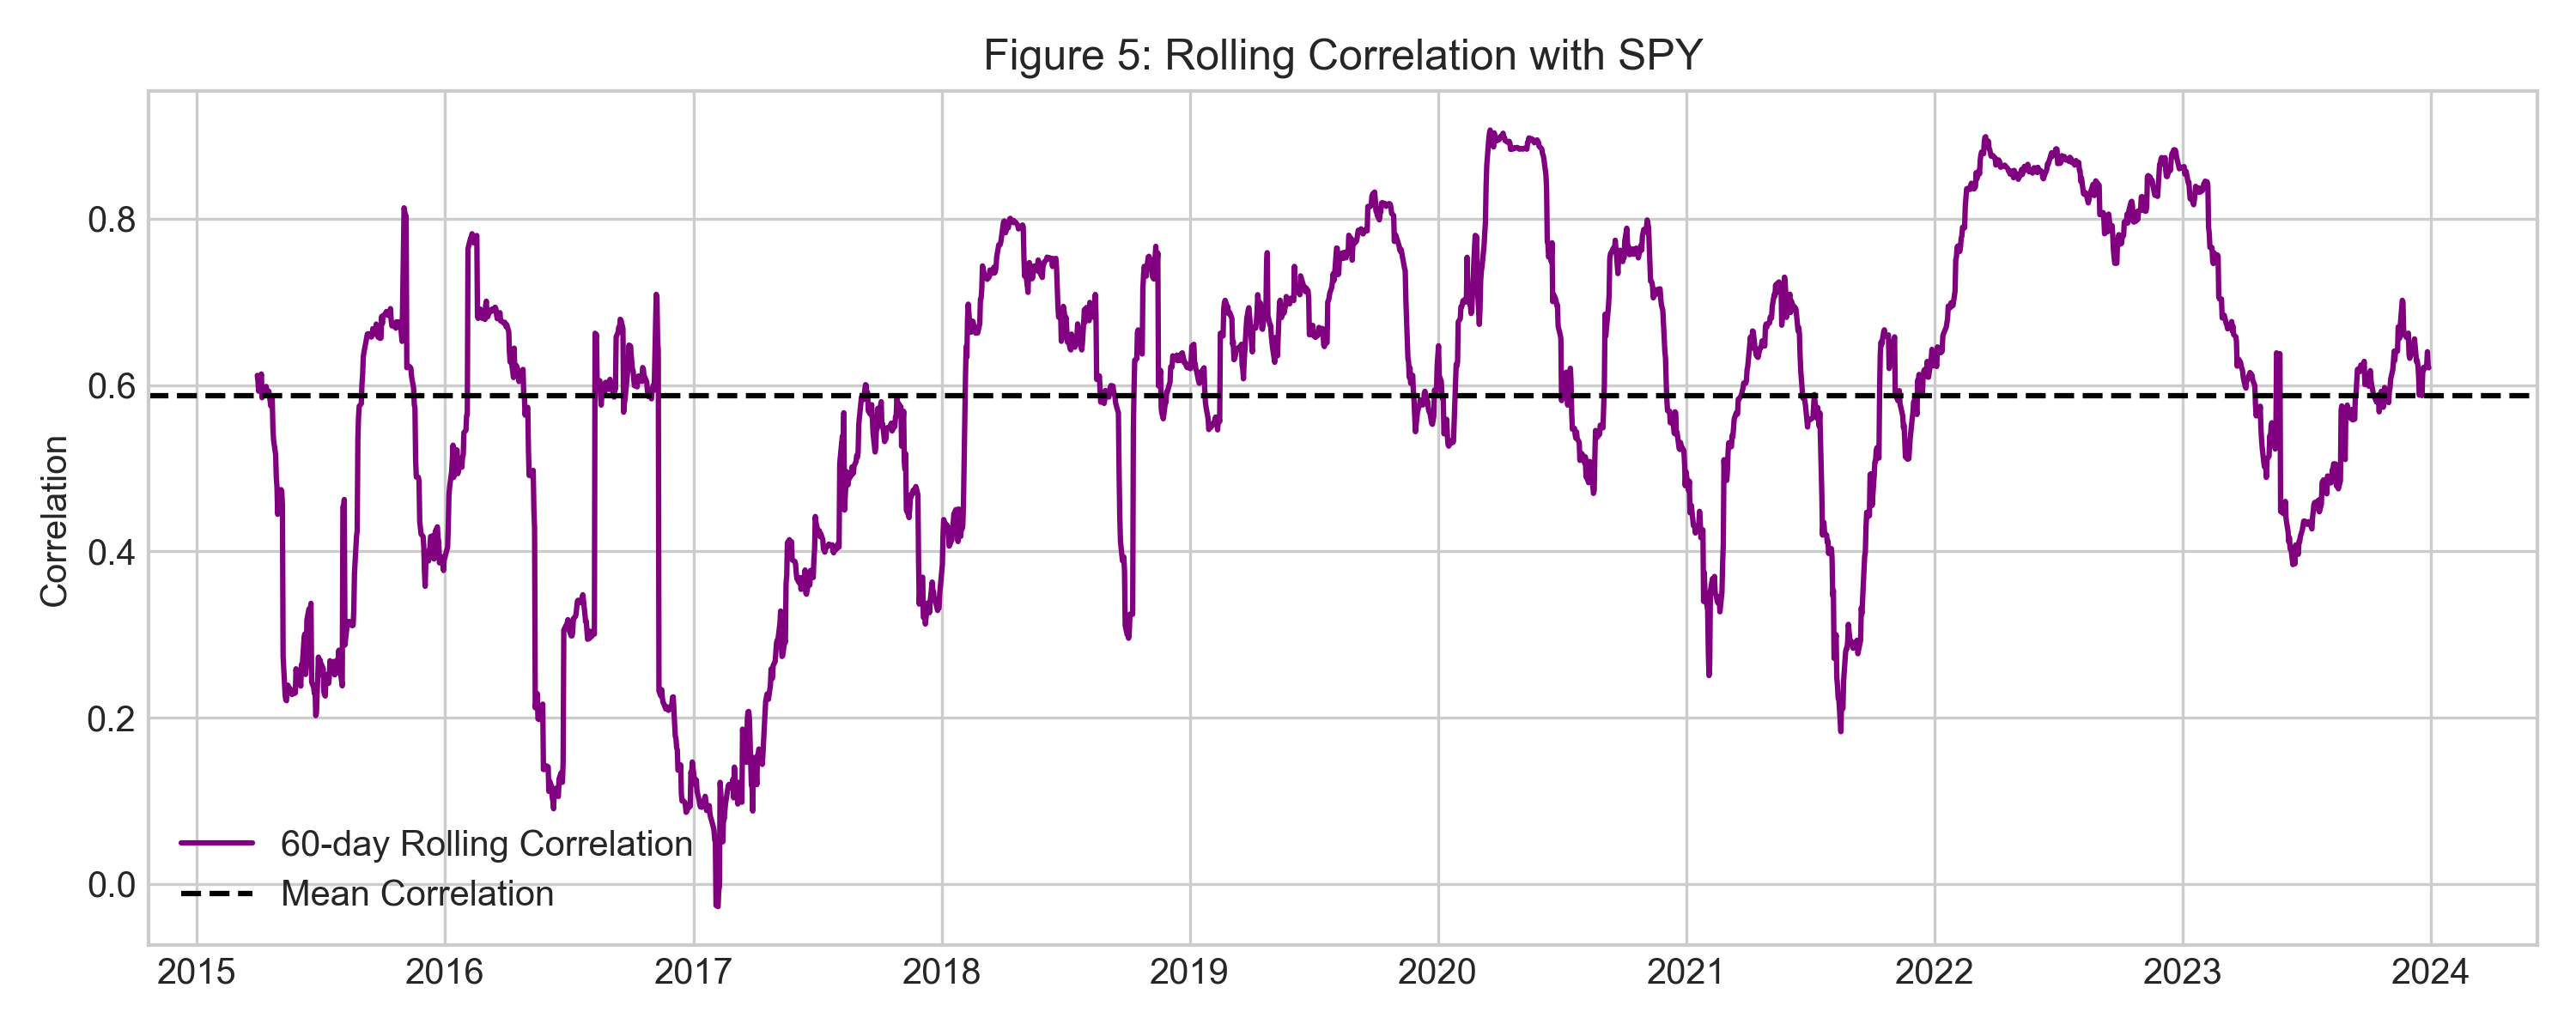
\includegraphics[width=0.8\textwidth]{eda_5_corr.png}
    \caption{Rolling 60-day Pearson Correlation matrix mapping idiosyncratic vs systematic shock propagation.}
\end{figure}

\begin{figure}[H]
    \centering
    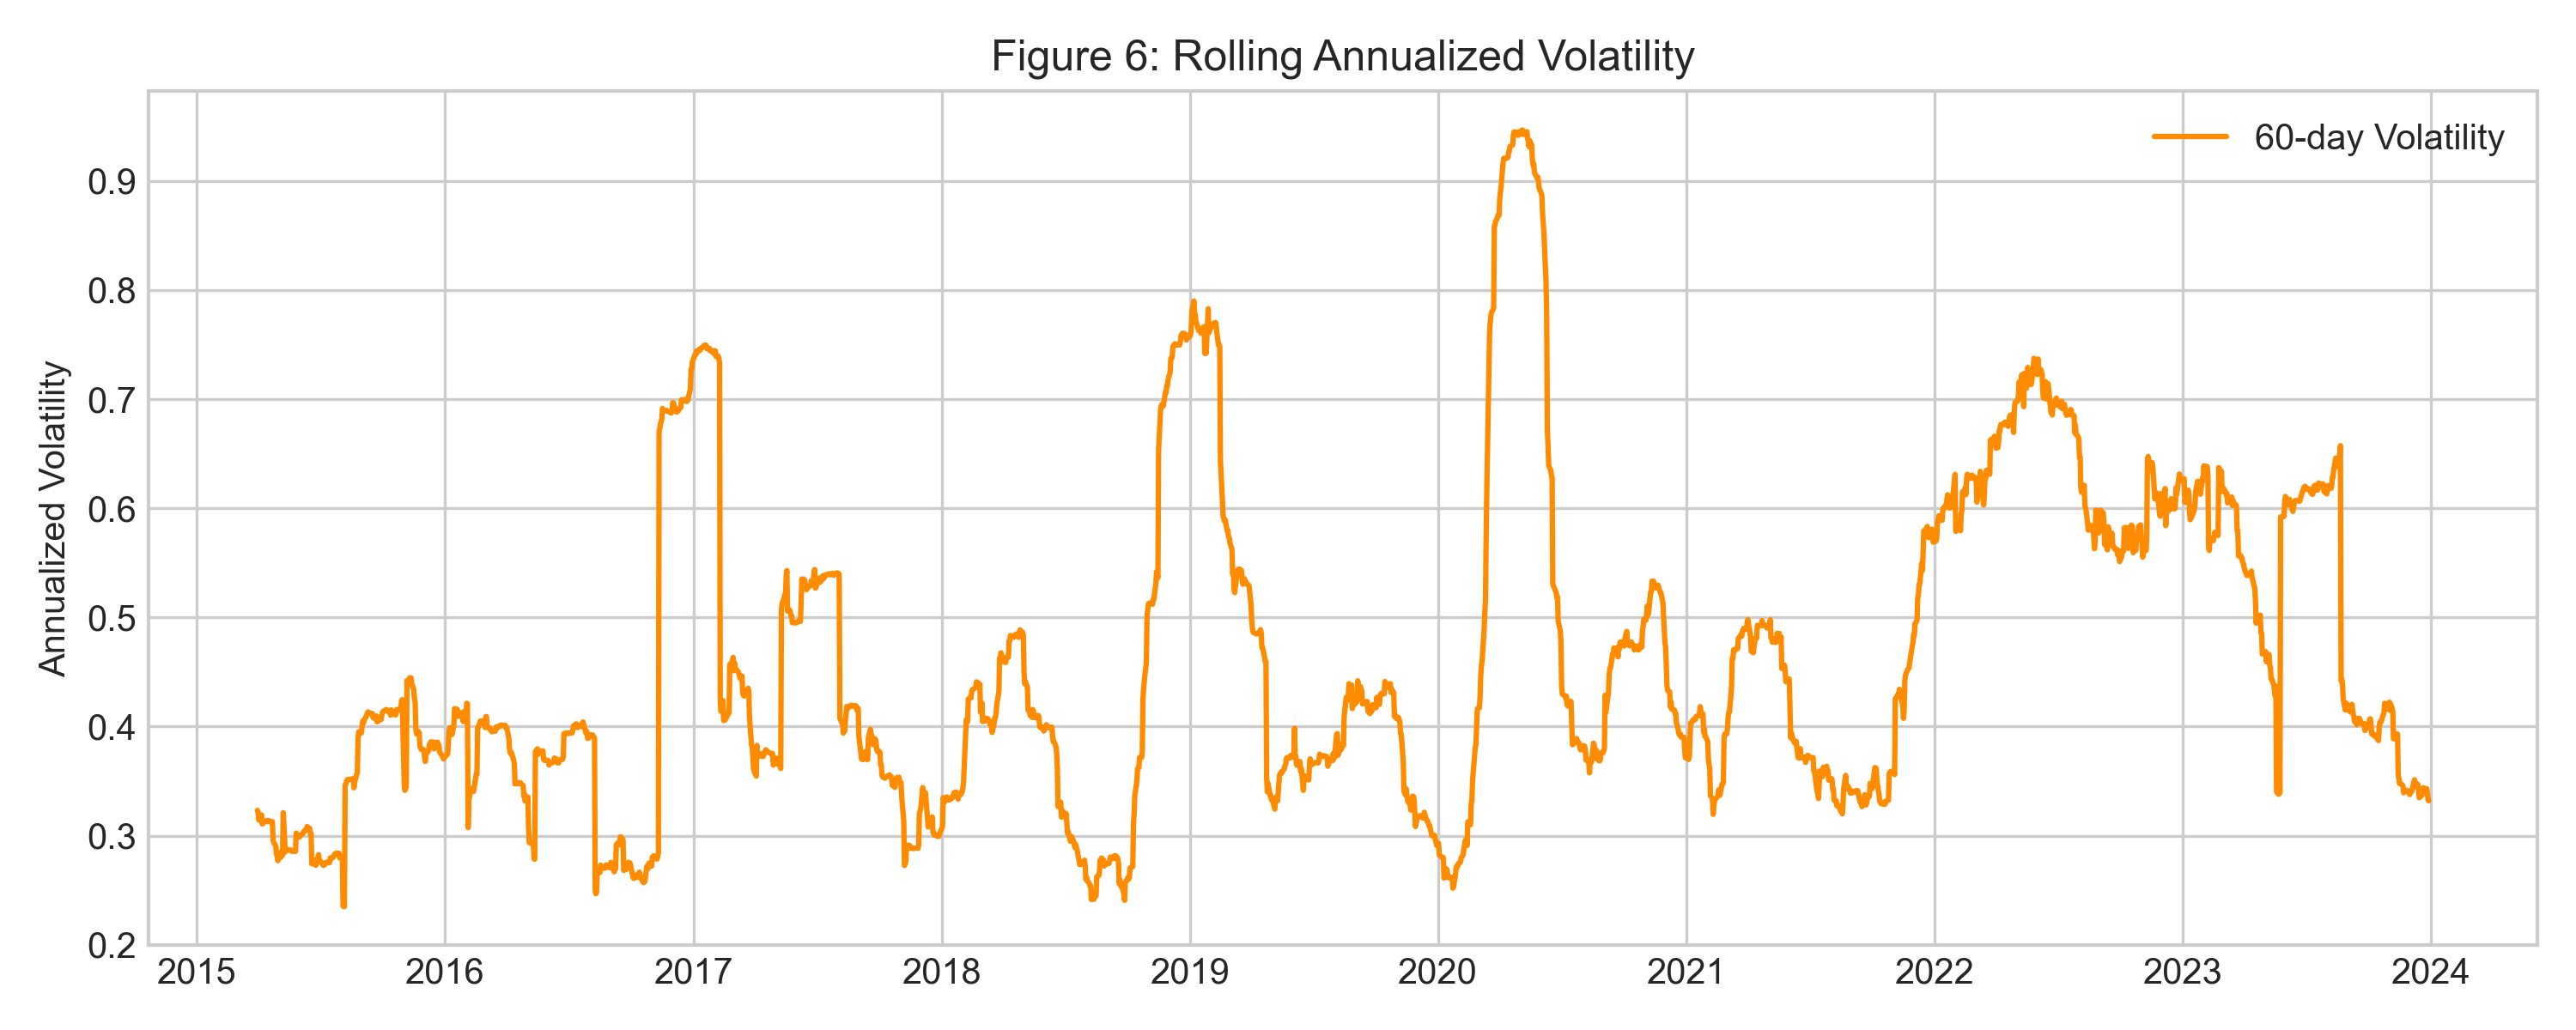
\includegraphics[width=0.8\textwidth]{eda_6_vol.png}
    \caption{Realized Volatility clustering phenomena proxying GARCH dynamics.}
\end{figure}
\section{Conclusion \& Academic Reflections}
. . . . . . . . . . . . . . . . . . . . . . . . . . . . . . . . . . . . . . . . . . . . . . . . . . . . . . . . . . . 19


\subsection{Summary of Findings . . . . . . . . . . . . . . . . . . . . . . . . . . . . . . . . . . . . . . . . . . . . . . . . . . . . . . . . . . . . . . . . . . . . 19}

\subsection{Critical Limitations \& Future Research . . . . . . . . . . . . . . . . . . . . . . . . . . . . . . . . . . . . . . . . . . . . . . . . . . . 19}



\end{document}
